\documentclass{book}
\usepackage[a4paper,top=2.5cm,bottom=2.5cm,left=2.5cm,right=2.5cm]{geometry}
\usepackage{makeidx}
\usepackage{natbib}
\usepackage{graphicx}
\usepackage{multicol}
\usepackage{float}
\usepackage{listings}
\usepackage{color}
\usepackage{ifthen}
\usepackage[table]{xcolor}
\usepackage{textcomp}
\usepackage{alltt}
\usepackage{ifpdf}
\ifpdf
\usepackage[pdftex,
            pagebackref=true,
            colorlinks=true,
            linkcolor=blue,
            unicode
           ]{hyperref}
\else
\usepackage[ps2pdf,
            pagebackref=true,
            colorlinks=true,
            linkcolor=blue,
            unicode
           ]{hyperref}
\usepackage{pspicture}
\fi
\usepackage[utf8]{inputenc}
\usepackage[brazil]{babel}
\usepackage{mathptmx}
\usepackage[scaled=.90]{helvet}
\usepackage{courier}
\usepackage{sectsty}
\usepackage[titles]{tocloft}
\usepackage{doxygen}
\lstset{language=C++,inputencoding=utf8,basicstyle=\footnotesize,breaklines=true,breakatwhitespace=true,tabsize=8,numbers=left }
\makeindex
\setcounter{tocdepth}{3}
\renewcommand{\footrulewidth}{0.4pt}
\renewcommand{\familydefault}{\sfdefault}
\hfuzz=15pt
\setlength{\emergencystretch}{15pt}
\hbadness=750
\tolerance=750
\begin{document}
\hypersetup{pageanchor=false,citecolor=blue}
\begin{titlepage}
\vspace*{7cm}
\begin{center}
{\Large Módulo de Física -\/ R\-K\-E }\\
\vspace*{1cm}
{\large Gerado por Doxygen 1.8.0}\\
\vspace*{0.5cm}
{\small Sexta, 18 de Maio de 2012 09:33:30}\\
\end{center}
\end{titlepage}
\clearemptydoublepage
\pagenumbering{roman}
\tableofcontents
\clearemptydoublepage
\pagenumbering{arabic}
\hypersetup{pageanchor=true,citecolor=blue}
\chapter{Índice dos Componentes}
\section{Estruturas de Dados}
Aqui estão as estruturas de dados, uniões e suas respectivas descrições\-:\begin{DoxyCompactList}
\item\contentsline{section}{\hyperlink{struct__jogador}{\-\_\-jogador} }{\pageref{struct__jogador}}{}
\item\contentsline{section}{\hyperlink{struct__ladrilho}{\-\_\-ladrilho} }{\pageref{struct__ladrilho}}{}
\item\contentsline{section}{\hyperlink{struct__objeto}{\-\_\-objeto} }{\pageref{struct__objeto}}{}
\item\contentsline{section}{\hyperlink{struct__tabuleiro}{\-\_\-tabuleiro} }{\pageref{struct__tabuleiro}}{}
\item\contentsline{section}{\hyperlink{structstruct__objeto}{struct\-\_\-objeto} }{\pageref{structstruct__objeto}}{}
\item\contentsline{section}{\hyperlink{structstruct__vetor}{struct\-\_\-vetor} }{\pageref{structstruct__vetor}}{}
\end{DoxyCompactList}

\chapter{Índice dos Arquivos}
\section{Lista de Arquivos}
Esta é a lista de todos os arquivos documentados e suas respectivas descrições\-:\begin{DoxyCompactList}
\item\contentsline{section}{include/\hyperlink{gunther_8h}{gunther.\-h} \\*Arquivo header geral do jogo }{\pageref{gunther_8h}}{}
\item\contentsline{section}{include/\hyperlink{rkefisica_8h}{rkefisica.\-h} \\*Arquivo header da biblioteca de funções físicas }{\pageref{rkefisica_8h}}{}
\item\contentsline{section}{include/\hyperlink{rkegraficos_8h}{rkegraficos.\-h} \\*Arquivo header da parte gráfica }{\pageref{rkegraficos_8h}}{}
\item\contentsline{section}{include/\hyperlink{rkerender_8h}{rkerender.\-h} \\*Arquivo header do renderizador }{\pageref{rkerender_8h}}{}
\item\contentsline{section}{include/\hyperlink{rketypes_8h}{rketypes.\-h} \\*Arquivo header de tipos e defines do Red Knife Engine }{\pageref{rketypes_8h}}{}
\item\contentsline{section}{src/\hyperlink{main_8c}{main.\-c} \\*Ponto de entrada do jogo }{\pageref{main_8c}}{}
\item\contentsline{section}{src/menu/\hyperlink{menu_8c}{menu.\-c} \\*Implementação do menu principal }{\pageref{menu_8c}}{}
\item\contentsline{section}{src/rkegraficos/\hyperlink{rkegraficos_8c}{rkegraficos.\-c} \\*Utilitários gráficos }{\pageref{rkegraficos_8c}}{}
\item\contentsline{section}{src/rkerender/\hyperlink{rkerender_8c}{rkerender.\-c} \\*Renderizador de fases }{\pageref{rkerender_8c}}{}
\end{DoxyCompactList}

\chapter{Classes}
\hypertarget{structstruct__objeto}{\section{Referência da Estrutura struct\-\_\-objeto}
\label{structstruct__objeto}\index{struct\-\_\-objeto@{struct\-\_\-objeto}}
}


{\ttfamily \#include $<$rketypes.\-h$>$}

\subsection*{Campos de Dados}
\begin{DoxyCompactItemize}
\item 
\hypertarget{structstruct__objeto_a7441ef0865bcb3db9b8064dd7375c1ea}{int {\bfseries id}}\label{structstruct__objeto_a7441ef0865bcb3db9b8064dd7375c1ea}

\item 
\hypertarget{structstruct__objeto_af88b946fb90d5f08b5fb740c70e98c10}{double {\bfseries x}}\label{structstruct__objeto_af88b946fb90d5f08b5fb740c70e98c10}

\item 
\hypertarget{structstruct__objeto_ab927965981178aa1fba979a37168db2a}{double {\bfseries y}}\label{structstruct__objeto_ab927965981178aa1fba979a37168db2a}

\item 
\hypertarget{structstruct__objeto_af8ea4d2851d2d656fd42be239e36ce6e}{double {\bfseries v\-\_\-x}}\label{structstruct__objeto_af8ea4d2851d2d656fd42be239e36ce6e}

\item 
\hypertarget{structstruct__objeto_a2161079bbf87834cfdf4d3548a53eb3b}{double {\bfseries v\-\_\-y}}\label{structstruct__objeto_a2161079bbf87834cfdf4d3548a53eb3b}

\item 
\hypertarget{structstruct__objeto_a3cb08d781a7ecc13047f1631906f7df5}{double {\bfseries massa}}\label{structstruct__objeto_a3cb08d781a7ecc13047f1631906f7df5}

\item 
\hypertarget{structstruct__objeto_aff2f6d52166217d13f9b2072c9e67c13}{double {\bfseries tempo}}\label{structstruct__objeto_aff2f6d52166217d13f9b2072c9e67c13}

\end{DoxyCompactItemize}


\subsection{Descrição Detalhada}
Struct objeto 
\begin{DoxyParams}{Parâmetros}
{\em id} & Identificador único \\
\hline
{\em x} & Componente x \\
\hline
{\em y} & Componente y \\
\hline
{\em v\-\_\-x} & Componente x da velocidade do objeto \\
\hline
{\em v\-\_\-y} & Componente y da velocidade do objeto \\
\hline
{\em massa} & Massa do objeto \\
\hline
{\em tempo} & Tempo de vida do objeto \\
\hline
\end{DoxyParams}


A documentação para esta estrutura foi gerada a partir do seguinte arquivo\-:\begin{DoxyCompactItemize}
\item 
include/\hyperlink{rketypes_8h}{rketypes.\-h}\end{DoxyCompactItemize}

\hypertarget{structstruct__vetor}{\section{struct\-\_\-vetor Struct Reference}
\label{structstruct__vetor}\index{struct\-\_\-vetor@{struct\-\_\-vetor}}
}


{\ttfamily \#include $<$rketypes.\-h$>$}

\subsection*{Public Attributes}
\begin{DoxyCompactItemize}
\item 
\hypertarget{structstruct__vetor_aae7646e904a8ce82b9c179ee26a0cc76}{double {\bfseries x}}\label{structstruct__vetor_aae7646e904a8ce82b9c179ee26a0cc76}

\item 
\hypertarget{structstruct__vetor_a73fafc2561b7eb18209e5ee4f6837b28}{double {\bfseries y}}\label{structstruct__vetor_a73fafc2561b7eb18209e5ee4f6837b28}

\end{DoxyCompactItemize}


\subsection{Detailed Description}
Struct vetor 
\begin{DoxyParams}{Parameters}
{\em x} & Componente x \\
\hline
{\em y} & Componente y \\
\hline
\end{DoxyParams}


The documentation for this struct was generated from the following file\-:\begin{DoxyCompactItemize}
\item 
include/\hyperlink{rketypes_8h}{rketypes.\-h}\end{DoxyCompactItemize}

\chapter{Arquivos}
\hypertarget{rkefisica_8h}{\section{Referência do Arquivo include/rkefisica.h}
\label{rkefisica_8h}\index{include/rkefisica.\-h@{include/rkefisica.\-h}}
}


Arquivo header da biblioteca de funções físicas.  


{\ttfamily \#include \char`\"{}rketypes.\-h\char`\"{}}\\*
Gráfico de dependência de inclusões para rkefisica.\-h\-:
Este grafo mostra quais arquivos estão direta ou indiretamente relacionados com este arquivo\-:
\subsection*{Funções}
\begin{DoxyCompactItemize}
\item 
void \hyperlink{rkefisica_8h_ae474cc3a29378896516478d39e1059b9}{rke\-\_\-set\-\_\-delta\-\_\-t} (double d\-\_\-t)
\item 
void \hyperlink{rkefisica_8h_ad9c136c98e2b18bb585f8c5b5c61152e}{rke\-\_\-set\-\_\-arrasto} (double coef\-\_\-arrasto)
\item 
void \hyperlink{rkefisica_8h_a4966d99bd4c2668b7d59a5e334330f86}{rke\-\_\-set\-\_\-vetor\-\_\-mundo} (double x, double y)
\item 
void \hyperlink{rkefisica_8h_ad669b81728dbf96d76dbed56981a3e84}{rke\-\_\-set\-\_\-numero\-\_\-objetos} (int numero)
\item 
void \hyperlink{rkefisica_8h_a4f887533c58a96b4cd5eff48ef195902}{rke\-\_\-adiciona\-\_\-objeto} (int id, double x, double y, double v\-\_\-x, double v\-\_\-y, double massa, double tempo)
\item 
\hyperlink{rketypes_8h_a216693704a51093135790527237245ec}{objeto} \hyperlink{rkefisica_8h_a3db469cd5f289d1376d1d27b53067875}{rke\-\_\-get\-\_\-objeto} (int i)
\item 
int \hyperlink{rkefisica_8h_a1c031c9197d9bfc50cdee27c0d8dd60a}{rke\-\_\-conta\-\_\-objetos} ()
\item 
void \hyperlink{rkefisica_8h_ae68fcd8b02679fe3b05c319820641449}{rke\-\_\-simula} ()
\end{DoxyCompactItemize}


\subsection{Descrição Detalhada}
Arquivo header da biblioteca de funções físicas. \begin{DoxyAuthor}{Autor}
João da Silva, Marina Salles, Ricardo Macedo 
\end{DoxyAuthor}


\subsection{Funções}
\hypertarget{rkefisica_8h_a4f887533c58a96b4cd5eff48ef195902}{\index{rkefisica.\-h@{rkefisica.\-h}!rke\-\_\-adiciona\-\_\-objeto@{rke\-\_\-adiciona\-\_\-objeto}}
\index{rke\-\_\-adiciona\-\_\-objeto@{rke\-\_\-adiciona\-\_\-objeto}!rkefisica.h@{rkefisica.\-h}}
\subsubsection[{rke\-\_\-adiciona\-\_\-objeto}]{\setlength{\rightskip}{0pt plus 5cm}void {\bf rke\-\_\-adiciona\-\_\-objeto} (
\begin{DoxyParamCaption}
\item[{int}]{id, }
\item[{double}]{x, }
\item[{double}]{y, }
\item[{double}]{v\-\_\-x, }
\item[{double}]{v\-\_\-y, }
\item[{double}]{massa, }
\item[{double}]{tempo}
\end{DoxyParamCaption}
)}}\label{rkefisica_8h_a4f887533c58a96b4cd5eff48ef195902}
Adiciona um objeto à lista de objetos a serem simulados. 
\begin{DoxyParams}{Parâmetros}
{\em id} & Identificador único do objeto \\
\hline
{\em x} & Posição x do objeto \\
\hline
{\em y} & Posição y do objeto \\
\hline
{\em v\-\_\-x} & Velocidade em x do objeto \\
\hline
{\em v\-\_\-y} & Velocidade em y do objeto \\
\hline
{\em massa} & Massa do objeto \\
\hline
{\em tempo} & Tempo de vida do objeto em segundos \\
\hline
\end{DoxyParams}
\hypertarget{rkefisica_8h_a1c031c9197d9bfc50cdee27c0d8dd60a}{\index{rkefisica.\-h@{rkefisica.\-h}!rke\-\_\-conta\-\_\-objetos@{rke\-\_\-conta\-\_\-objetos}}
\index{rke\-\_\-conta\-\_\-objetos@{rke\-\_\-conta\-\_\-objetos}!rkefisica.h@{rkefisica.\-h}}
\subsubsection[{rke\-\_\-conta\-\_\-objetos}]{\setlength{\rightskip}{0pt plus 5cm}int {\bf rke\-\_\-conta\-\_\-objetos} (
\begin{DoxyParamCaption}
{}
\end{DoxyParamCaption}
)}}\label{rkefisica_8h_a1c031c9197d9bfc50cdee27c0d8dd60a}
Conta o número de objetos ativos, ou seja, com tempo de vida diferente de zero. \hypertarget{rkefisica_8h_a3db469cd5f289d1376d1d27b53067875}{\index{rkefisica.\-h@{rkefisica.\-h}!rke\-\_\-get\-\_\-objeto@{rke\-\_\-get\-\_\-objeto}}
\index{rke\-\_\-get\-\_\-objeto@{rke\-\_\-get\-\_\-objeto}!rkefisica.h@{rkefisica.\-h}}
\subsubsection[{rke\-\_\-get\-\_\-objeto}]{\setlength{\rightskip}{0pt plus 5cm}{\bf objeto} {\bf rke\-\_\-get\-\_\-objeto} (
\begin{DoxyParamCaption}
\item[{int}]{i}
\end{DoxyParamCaption}
)}}\label{rkefisica_8h_a3db469cd5f289d1376d1d27b53067875}
Retorna o i-\/ésimo objeto. 
\begin{DoxyParams}{Parâmetros}
{\em i} & Índice do objeto \\
\hline
\end{DoxyParams}
\hypertarget{rkefisica_8h_ad9c136c98e2b18bb585f8c5b5c61152e}{\index{rkefisica.\-h@{rkefisica.\-h}!rke\-\_\-set\-\_\-arrasto@{rke\-\_\-set\-\_\-arrasto}}
\index{rke\-\_\-set\-\_\-arrasto@{rke\-\_\-set\-\_\-arrasto}!rkefisica.h@{rkefisica.\-h}}
\subsubsection[{rke\-\_\-set\-\_\-arrasto}]{\setlength{\rightskip}{0pt plus 5cm}void {\bf rke\-\_\-set\-\_\-arrasto} (
\begin{DoxyParamCaption}
\item[{double}]{coef\-\_\-arrasto}
\end{DoxyParamCaption}
)}}\label{rkefisica_8h_ad9c136c98e2b18bb585f8c5b5c61152e}
Configura o coeficiente de arrasto da superfície. 
\begin{DoxyParams}{Parâmetros}
{\em coef\-\_\-arrasto} & Coeficiente de 0.\-0 a 1.\-0 \\
\hline
\end{DoxyParams}
\hypertarget{rkefisica_8h_ae474cc3a29378896516478d39e1059b9}{\index{rkefisica.\-h@{rkefisica.\-h}!rke\-\_\-set\-\_\-delta\-\_\-t@{rke\-\_\-set\-\_\-delta\-\_\-t}}
\index{rke\-\_\-set\-\_\-delta\-\_\-t@{rke\-\_\-set\-\_\-delta\-\_\-t}!rkefisica.h@{rkefisica.\-h}}
\subsubsection[{rke\-\_\-set\-\_\-delta\-\_\-t}]{\setlength{\rightskip}{0pt plus 5cm}void {\bf rke\-\_\-set\-\_\-delta\-\_\-t} (
\begin{DoxyParamCaption}
\item[{double}]{d\-\_\-t}
\end{DoxyParamCaption}
)}}\label{rkefisica_8h_ae474cc3a29378896516478d39e1059b9}
Indica a resolução da simulação. Este é o tamanho do quanta de tempo. 
\begin{DoxyParams}{Parâmetros}
{\em d\-\_\-t} & Resolução em segundos \\
\hline
\end{DoxyParams}
\hypertarget{rkefisica_8h_ad669b81728dbf96d76dbed56981a3e84}{\index{rkefisica.\-h@{rkefisica.\-h}!rke\-\_\-set\-\_\-numero\-\_\-objetos@{rke\-\_\-set\-\_\-numero\-\_\-objetos}}
\index{rke\-\_\-set\-\_\-numero\-\_\-objetos@{rke\-\_\-set\-\_\-numero\-\_\-objetos}!rkefisica.h@{rkefisica.\-h}}
\subsubsection[{rke\-\_\-set\-\_\-numero\-\_\-objetos}]{\setlength{\rightskip}{0pt plus 5cm}void {\bf rke\-\_\-set\-\_\-numero\-\_\-objetos} (
\begin{DoxyParamCaption}
\item[{int}]{numero}
\end{DoxyParamCaption}
)}}\label{rkefisica_8h_ad669b81728dbf96d76dbed56981a3e84}
Configura o número total de objetos a serem simulados. 
\begin{DoxyParams}{Parâmetros}
{\em numero} & Número de objetos \\
\hline
\end{DoxyParams}
\hypertarget{rkefisica_8h_a4966d99bd4c2668b7d59a5e334330f86}{\index{rkefisica.\-h@{rkefisica.\-h}!rke\-\_\-set\-\_\-vetor\-\_\-mundo@{rke\-\_\-set\-\_\-vetor\-\_\-mundo}}
\index{rke\-\_\-set\-\_\-vetor\-\_\-mundo@{rke\-\_\-set\-\_\-vetor\-\_\-mundo}!rkefisica.h@{rkefisica.\-h}}
\subsubsection[{rke\-\_\-set\-\_\-vetor\-\_\-mundo}]{\setlength{\rightskip}{0pt plus 5cm}void {\bf rke\-\_\-set\-\_\-vetor\-\_\-mundo} (
\begin{DoxyParamCaption}
\item[{double}]{x, }
\item[{double}]{y}
\end{DoxyParamCaption}
)}}\label{rkefisica_8h_a4966d99bd4c2668b7d59a5e334330f86}
Configura o vetor base que regirá todos os objetos do mundo. 
\begin{DoxyParams}{Parâmetros}
{\em x} & Componente x \\
\hline
{\em y} & Componente y \\
\hline
\end{DoxyParams}
\hypertarget{rkefisica_8h_ae68fcd8b02679fe3b05c319820641449}{\index{rkefisica.\-h@{rkefisica.\-h}!rke\-\_\-simula@{rke\-\_\-simula}}
\index{rke\-\_\-simula@{rke\-\_\-simula}!rkefisica.h@{rkefisica.\-h}}
\subsubsection[{rke\-\_\-simula}]{\setlength{\rightskip}{0pt plus 5cm}void {\bf rke\-\_\-simula} (
\begin{DoxyParamCaption}
{}
\end{DoxyParamCaption}
)}}\label{rkefisica_8h_ae68fcd8b02679fe3b05c319820641449}
Simula todos os objetos por um quanta de tempo. 
\hypertarget{rketypes_8h}{
\section{Referência do Arquivo bkp/rketypes.h}
\label{rketypes_8h}\index{bkp/rketypes.h@{bkp/rketypes.h}}
}


Arquivo header de tipos e defines do Red Knife Engine.  


Este grafo mostra quais arquivos estão direta ou indiretamente relacionados com este arquivo:
\nopagebreak
\begin{figure}[H]
\begin{center}
\leavevmode
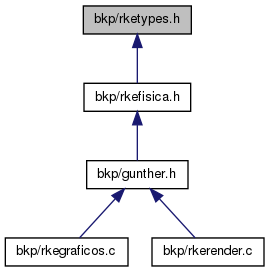
\includegraphics[width=274pt]{rketypes_8h__dep__incl}
\end{center}
\end{figure}
\subsection*{Estruturas de Dados}
\begin{DoxyCompactItemize}
\item 
struct \hyperlink{structstruct__vetor}{struct\_\-vetor}
\item 
struct \hyperlink{structstruct__objeto}{struct\_\-objeto}
\end{DoxyCompactItemize}
\subsection*{Definições e Macros}
\begin{DoxyCompactItemize}
\item 
\hypertarget{rketypes_8h_a446118036aeca9a42bc2d451ab80b8b7}{
\#define {\bfseries BARCOID}~-\/1}
\label{rketypes_8h_a446118036aeca9a42bc2d451ab80b8b7}

\item 
\hypertarget{rketypes_8h_a58883c467f961c4b1f998d575f943890}{
\#define {\bfseries ESTATICO}~-\/1.0}
\label{rketypes_8h_a58883c467f961c4b1f998d575f943890}

\end{DoxyCompactItemize}
\subsection*{Definições de Tipos}
\begin{DoxyCompactItemize}
\item 
typedef struct \hyperlink{structstruct__vetor}{struct\_\-vetor} \hyperlink{rketypes_8h_a27896866572b2a12760a22ea2654ed47}{vetor}
\item 
typedef struct \hyperlink{structstruct__objeto}{struct\_\-objeto} \hyperlink{rketypes_8h_a216693704a51093135790527237245ec}{objeto}
\end{DoxyCompactItemize}


\subsection{Descrição Detalhada}
Arquivo header de tipos e defines do Red Knife Engine. \begin{DoxyAuthor}{Autor}
João da Silva, Marina Salles, Ricardo Macedo 
\end{DoxyAuthor}


\subsection{Definições dos tipos}
\hypertarget{rketypes_8h_a216693704a51093135790527237245ec}{
\index{rketypes.h@{rketypes.h}!objeto@{objeto}}
\index{objeto@{objeto}!rketypes.h@{rketypes.h}}
\subsubsection[{objeto}]{\setlength{\rightskip}{0pt plus 5cm}typedef struct {\bf struct\_\-objeto}  {\bf objeto}}}
\label{rketypes_8h_a216693704a51093135790527237245ec}
Struct objeto 
\begin{DoxyParams}{Parâmetros}
{\em id} & Identificador único \\
\hline
{\em x} & Componente x \\
\hline
{\em y} & Componente y \\
\hline
{\em v\_\-x} & Componente x da velocidade do objeto \\
\hline
{\em v\_\-y} & Componente y da velocidade do objeto \\
\hline
{\em massa} & Massa do objeto \\
\hline
{\em tempo} & Tempo de vida do objeto \\
\hline
\end{DoxyParams}
\hypertarget{rketypes_8h_a27896866572b2a12760a22ea2654ed47}{
\index{rketypes.h@{rketypes.h}!vetor@{vetor}}
\index{vetor@{vetor}!rketypes.h@{rketypes.h}}
\subsubsection[{vetor}]{\setlength{\rightskip}{0pt plus 5cm}typedef struct {\bf struct\_\-vetor}  {\bf vetor}}}
\label{rketypes_8h_a27896866572b2a12760a22ea2654ed47}
Struct vetor 
\begin{DoxyParams}{Parâmetros}
{\em x} & Componente x \\
\hline
{\em y} & Componente y \\
\hline
\end{DoxyParams}

\hypertarget{fisica_8c}{\section{Referência do Arquivo src/fisica.c}
\label{fisica_8c}\index{src/fisica.\-c@{src/fisica.\-c}}
}


Esta é a biblioteca de funções que lidam com a física do Red Knife Engine.  


{\ttfamily \#include $<$stdio.\-h$>$}\\*
{\ttfamily \#include $<$stdlib.\-h$>$}\\*
{\ttfamily \#include $<$math.\-h$>$}\\*
{\ttfamily \#include \char`\"{}../include/rketypes.\-h\char`\"{}}\\*
Gráfico de dependência de inclusões para fisica.\-c\-:
\subsection*{Funções}
\begin{DoxyCompactItemize}
\item 
void \hyperlink{fisica_8c_ae474cc3a29378896516478d39e1059b9}{rke\-\_\-set\-\_\-delta\-\_\-t} (double d\-\_\-t)
\item 
void \hyperlink{fisica_8c_ad9c136c98e2b18bb585f8c5b5c61152e}{rke\-\_\-set\-\_\-arrasto} (double coef\-\_\-arrasto)
\item 
void \hyperlink{fisica_8c_a4966d99bd4c2668b7d59a5e334330f86}{rke\-\_\-set\-\_\-vetor\-\_\-mundo} (double x, double y)
\item 
void \hyperlink{fisica_8c_ad669b81728dbf96d76dbed56981a3e84}{rke\-\_\-set\-\_\-numero\-\_\-objetos} (int numero)
\item 
void \hyperlink{fisica_8c_a4e96e803ac19354b2b63dd14a5f5e67d}{itera\-\_\-posicao} (\hyperlink{rketypes_8h_a216693704a51093135790527237245ec}{objeto} $\ast$obj, \hyperlink{rketypes_8h_a27896866572b2a12760a22ea2654ed47}{vetor} forca)
\item 
void \hyperlink{fisica_8c_a4f887533c58a96b4cd5eff48ef195902}{rke\-\_\-adiciona\-\_\-objeto} (int id, double x, double y, double v\-\_\-x, double v\-\_\-y, double massa, double tempo)
\item 
\hyperlink{rketypes_8h_a216693704a51093135790527237245ec}{objeto} \hyperlink{fisica_8c_a3db469cd5f289d1376d1d27b53067875}{rke\-\_\-get\-\_\-objeto} (int i)
\item 
void \hyperlink{fisica_8c_ae68fcd8b02679fe3b05c319820641449}{rke\-\_\-simula} ()
\end{DoxyCompactItemize}
\subsection*{Variáveis}
\begin{DoxyCompactItemize}
\item 
\hypertarget{fisica_8c_a4cfc079302fe9a34fe24637c4e44303a}{double {\bfseries delta\-\_\-t}}\label{fisica_8c_a4cfc079302fe9a34fe24637c4e44303a}

\item 
\hypertarget{fisica_8c_a26ef23742f66901f318f34e704586fa4}{double {\bfseries percentual\-\_\-atrito}}\label{fisica_8c_a26ef23742f66901f318f34e704586fa4}

\item 
\hypertarget{fisica_8c_a9b2b25a25c5da642c3c370b168392147}{double {\bfseries arrasto}}\label{fisica_8c_a9b2b25a25c5da642c3c370b168392147}

\item 
\hypertarget{fisica_8c_a499879a953d3f4c7cc580c150d6bedc5}{\hyperlink{rketypes_8h_a27896866572b2a12760a22ea2654ed47}{vetor} {\bfseries mundo}}\label{fisica_8c_a499879a953d3f4c7cc580c150d6bedc5}

\item 
\hypertarget{fisica_8c_a96d3b7bc41d3291ebe52930441134b04}{int {\bfseries ult\-\_\-objeto} = 0}\label{fisica_8c_a96d3b7bc41d3291ebe52930441134b04}

\item 
\hypertarget{fisica_8c_a94e5b9e80fdd9036dbb049ba24e067da}{int {\bfseries num\-\_\-objetos} = 0}\label{fisica_8c_a94e5b9e80fdd9036dbb049ba24e067da}

\item 
\hypertarget{fisica_8c_a87c3c30ca18c98a0d848c580f53ad49f}{\hyperlink{rketypes_8h_a216693704a51093135790527237245ec}{objeto} $\ast$ {\bfseries objetos}}\label{fisica_8c_a87c3c30ca18c98a0d848c580f53ad49f}

\end{DoxyCompactItemize}


\subsection{Descrição Detalhada}
Esta é a biblioteca de funções que lidam com a física do Red Knife Engine. \begin{DoxyAuthor}{Autor}
João da Silva, Marina Salles, Ricardo Macedo 
\end{DoxyAuthor}


\subsection{Funções}
\hypertarget{fisica_8c_a4e96e803ac19354b2b63dd14a5f5e67d}{\index{fisica.\-c@{fisica.\-c}!itera\-\_\-posicao@{itera\-\_\-posicao}}
\index{itera\-\_\-posicao@{itera\-\_\-posicao}!fisica.c@{fisica.\-c}}
\subsubsection[{itera\-\_\-posicao}]{\setlength{\rightskip}{0pt plus 5cm}void {\bf itera\-\_\-posicao} (
\begin{DoxyParamCaption}
\item[{{\bf objeto} $\ast$}]{obj, }
\item[{{\bf vetor}}]{forca}
\end{DoxyParamCaption}
)}}\label{fisica_8c_a4e96e803ac19354b2b63dd14a5f5e67d}
De acordo com a velocidade do objeto, o tempo de vida dele, o vetor mundo e a massa, calcula a posição seguinte no próximo quanta de tempo. 
\begin{DoxyParams}{Parâmetros}
{\em obj} & Endereço do objeto \\
\hline
{\em forca} & Força a ser aplicada \\
\hline
\end{DoxyParams}
\hypertarget{fisica_8c_a4f887533c58a96b4cd5eff48ef195902}{\index{fisica.\-c@{fisica.\-c}!rke\-\_\-adiciona\-\_\-objeto@{rke\-\_\-adiciona\-\_\-objeto}}
\index{rke\-\_\-adiciona\-\_\-objeto@{rke\-\_\-adiciona\-\_\-objeto}!fisica.c@{fisica.\-c}}
\subsubsection[{rke\-\_\-adiciona\-\_\-objeto}]{\setlength{\rightskip}{0pt plus 5cm}void {\bf rke\-\_\-adiciona\-\_\-objeto} (
\begin{DoxyParamCaption}
\item[{int}]{id, }
\item[{double}]{x, }
\item[{double}]{y, }
\item[{double}]{v\-\_\-x, }
\item[{double}]{v\-\_\-y, }
\item[{double}]{massa, }
\item[{double}]{tempo}
\end{DoxyParamCaption}
)}}\label{fisica_8c_a4f887533c58a96b4cd5eff48ef195902}
Adiciona um objeto à lista de objetos a serem simulados. 
\begin{DoxyParams}{Parâmetros}
{\em id} & Identificador único do objeto \\
\hline
{\em x} & Posição x do objeto \\
\hline
{\em y} & Posição y do objeto \\
\hline
{\em v\-\_\-x} & Velocidade em x do objeto \\
\hline
{\em v\-\_\-y} & Velocidade em y do objeto \\
\hline
{\em massa} & Massa do objeto \\
\hline
{\em tempo} & Tempo de vida do objeto em segundos \\
\hline
\end{DoxyParams}
\hypertarget{fisica_8c_a3db469cd5f289d1376d1d27b53067875}{\index{fisica.\-c@{fisica.\-c}!rke\-\_\-get\-\_\-objeto@{rke\-\_\-get\-\_\-objeto}}
\index{rke\-\_\-get\-\_\-objeto@{rke\-\_\-get\-\_\-objeto}!fisica.c@{fisica.\-c}}
\subsubsection[{rke\-\_\-get\-\_\-objeto}]{\setlength{\rightskip}{0pt plus 5cm}{\bf objeto} {\bf rke\-\_\-get\-\_\-objeto} (
\begin{DoxyParamCaption}
\item[{int}]{i}
\end{DoxyParamCaption}
)}}\label{fisica_8c_a3db469cd5f289d1376d1d27b53067875}
Retorna o i-\/ésimo objeto. 
\begin{DoxyParams}{Parâmetros}
{\em i} & Índice do objeto \\
\hline
\end{DoxyParams}
\hypertarget{fisica_8c_ad9c136c98e2b18bb585f8c5b5c61152e}{\index{fisica.\-c@{fisica.\-c}!rke\-\_\-set\-\_\-arrasto@{rke\-\_\-set\-\_\-arrasto}}
\index{rke\-\_\-set\-\_\-arrasto@{rke\-\_\-set\-\_\-arrasto}!fisica.c@{fisica.\-c}}
\subsubsection[{rke\-\_\-set\-\_\-arrasto}]{\setlength{\rightskip}{0pt plus 5cm}void {\bf rke\-\_\-set\-\_\-arrasto} (
\begin{DoxyParamCaption}
\item[{double}]{coef\-\_\-arrasto}
\end{DoxyParamCaption}
)}}\label{fisica_8c_ad9c136c98e2b18bb585f8c5b5c61152e}
Configura o coeficiente de arrasto da superfície. 
\begin{DoxyParams}{Parâmetros}
{\em coef\-\_\-arrasto} & Coeficiente de 0.\-0 a 1.\-0 \\
\hline
\end{DoxyParams}
\hypertarget{fisica_8c_ae474cc3a29378896516478d39e1059b9}{\index{fisica.\-c@{fisica.\-c}!rke\-\_\-set\-\_\-delta\-\_\-t@{rke\-\_\-set\-\_\-delta\-\_\-t}}
\index{rke\-\_\-set\-\_\-delta\-\_\-t@{rke\-\_\-set\-\_\-delta\-\_\-t}!fisica.c@{fisica.\-c}}
\subsubsection[{rke\-\_\-set\-\_\-delta\-\_\-t}]{\setlength{\rightskip}{0pt plus 5cm}void {\bf rke\-\_\-set\-\_\-delta\-\_\-t} (
\begin{DoxyParamCaption}
\item[{double}]{d\-\_\-t}
\end{DoxyParamCaption}
)}}\label{fisica_8c_ae474cc3a29378896516478d39e1059b9}
Indica a resolução da simulação. Este é o tamanho do quanta de tempo. 
\begin{DoxyParams}{Parâmetros}
{\em d\-\_\-t} & Resolução em segundos \\
\hline
\end{DoxyParams}
\hypertarget{fisica_8c_ad669b81728dbf96d76dbed56981a3e84}{\index{fisica.\-c@{fisica.\-c}!rke\-\_\-set\-\_\-numero\-\_\-objetos@{rke\-\_\-set\-\_\-numero\-\_\-objetos}}
\index{rke\-\_\-set\-\_\-numero\-\_\-objetos@{rke\-\_\-set\-\_\-numero\-\_\-objetos}!fisica.c@{fisica.\-c}}
\subsubsection[{rke\-\_\-set\-\_\-numero\-\_\-objetos}]{\setlength{\rightskip}{0pt plus 5cm}void {\bf rke\-\_\-set\-\_\-numero\-\_\-objetos} (
\begin{DoxyParamCaption}
\item[{int}]{numero}
\end{DoxyParamCaption}
)}}\label{fisica_8c_ad669b81728dbf96d76dbed56981a3e84}
Configura o número total de objetos a serem simulados. 
\begin{DoxyParams}{Parâmetros}
{\em numero} & Número de objetos \\
\hline
\end{DoxyParams}
\hypertarget{fisica_8c_a4966d99bd4c2668b7d59a5e334330f86}{\index{fisica.\-c@{fisica.\-c}!rke\-\_\-set\-\_\-vetor\-\_\-mundo@{rke\-\_\-set\-\_\-vetor\-\_\-mundo}}
\index{rke\-\_\-set\-\_\-vetor\-\_\-mundo@{rke\-\_\-set\-\_\-vetor\-\_\-mundo}!fisica.c@{fisica.\-c}}
\subsubsection[{rke\-\_\-set\-\_\-vetor\-\_\-mundo}]{\setlength{\rightskip}{0pt plus 5cm}void {\bf rke\-\_\-set\-\_\-vetor\-\_\-mundo} (
\begin{DoxyParamCaption}
\item[{double}]{x, }
\item[{double}]{y}
\end{DoxyParamCaption}
)}}\label{fisica_8c_a4966d99bd4c2668b7d59a5e334330f86}
Configura o vetor base que regirá todos os objetos do mundo. 
\begin{DoxyParams}{Parâmetros}
{\em x} & Componente x \\
\hline
{\em y} & Componente y \\
\hline
\end{DoxyParams}
\hypertarget{fisica_8c_ae68fcd8b02679fe3b05c319820641449}{\index{fisica.\-c@{fisica.\-c}!rke\-\_\-simula@{rke\-\_\-simula}}
\index{rke\-\_\-simula@{rke\-\_\-simula}!fisica.c@{fisica.\-c}}
\subsubsection[{rke\-\_\-simula}]{\setlength{\rightskip}{0pt plus 5cm}void {\bf rke\-\_\-simula} (
\begin{DoxyParamCaption}
{}
\end{DoxyParamCaption}
)}}\label{fisica_8c_ae68fcd8b02679fe3b05c319820641449}
Simula todos os objetos por um quanta de tempo. 
\hypertarget{main_8c}{\section{src/main.c File Reference}
\label{main_8c}\index{src/main.\-c@{src/main.\-c}}
}


Este é o arquivo que implementa as funções descritas na \hyperlink{fisica_8c}{fisica.\-c}. Aqui, carrega-\/se um arquivo texto com as condições iniciais e escreve um arquivo \char`\"{}saida.\-out\char`\"{} com as informações após as iterações.  


{\ttfamily \#include $<$stdio.\-h$>$}\\*
{\ttfamily \#include $<$stdlib.\-h$>$}\\*
{\ttfamily \#include $<$string.\-h$>$}\\*
{\ttfamily \#include \char`\"{}../include/rketypes.\-h\char`\"{}}\\*
{\ttfamily \#include \char`\"{}../include/rkefisica.\-h\char`\"{}}\\*
Include dependency graph for main.\-c\-:
\subsection*{Functions}
\begin{DoxyCompactItemize}
\item 
\hypertarget{main_8c_a0ddf1224851353fc92bfbff6f499fa97}{int {\bfseries main} (int argc, char $\ast$argv\mbox{[}$\,$\mbox{]})}\label{main_8c_a0ddf1224851353fc92bfbff6f499fa97}

\end{DoxyCompactItemize}


\subsection{Detailed Description}
Este é o arquivo que implementa as funções descritas na \hyperlink{fisica_8c}{fisica.\-c}. Aqui, carrega-\/se um arquivo texto com as condições iniciais e escreve um arquivo \char`\"{}saida.\-out\char`\"{} com as informações após as iterações. \begin{DoxyAuthor}{Author}
João da Silva, Marina Salles, Ricardo Macedo 
\end{DoxyAuthor}

\printindex
\end{document}
